\section{Estimating (Small-Scale) Scaling Laws}
\label{sec:estimating-small-scale-scaling-laws}

In this study, we will use models ranging in size from 4--34M to estimate scaling laws, 67M--134M for validation, and 268M for testing.
All details about the experimental design chosen in this study are in Appendix~\ref{app:experimental-design}.

What does it take to estimate scaling laws from small-scale experiments? We find them fairly robust to different decisions (\S\ref{sec:estimating-small-scale-scaling-laws:the-impact-of-methodology}), but one ingredient makes or breaks the resulting law: hyperparameter tuning (\S\ref{sec:estimating-small-scale-scaling-laws:the-importance-of-hyperparameter-tuning}).

\subsection{The Impact of Methodology}
\label{sec:estimating-small-scale-scaling-laws:the-impact-of-methodology}

Despite the frequent debate over parameter definitions, we find they make little difference. Beyond that, we study three refinements on a basic approach: tuning hyperparameters per token budget, decaying the learning rate, and tying the scaling exponents. Some help but none, we will see, is what makes the estimate work.

\begin{figure}[t!]
    \centering
    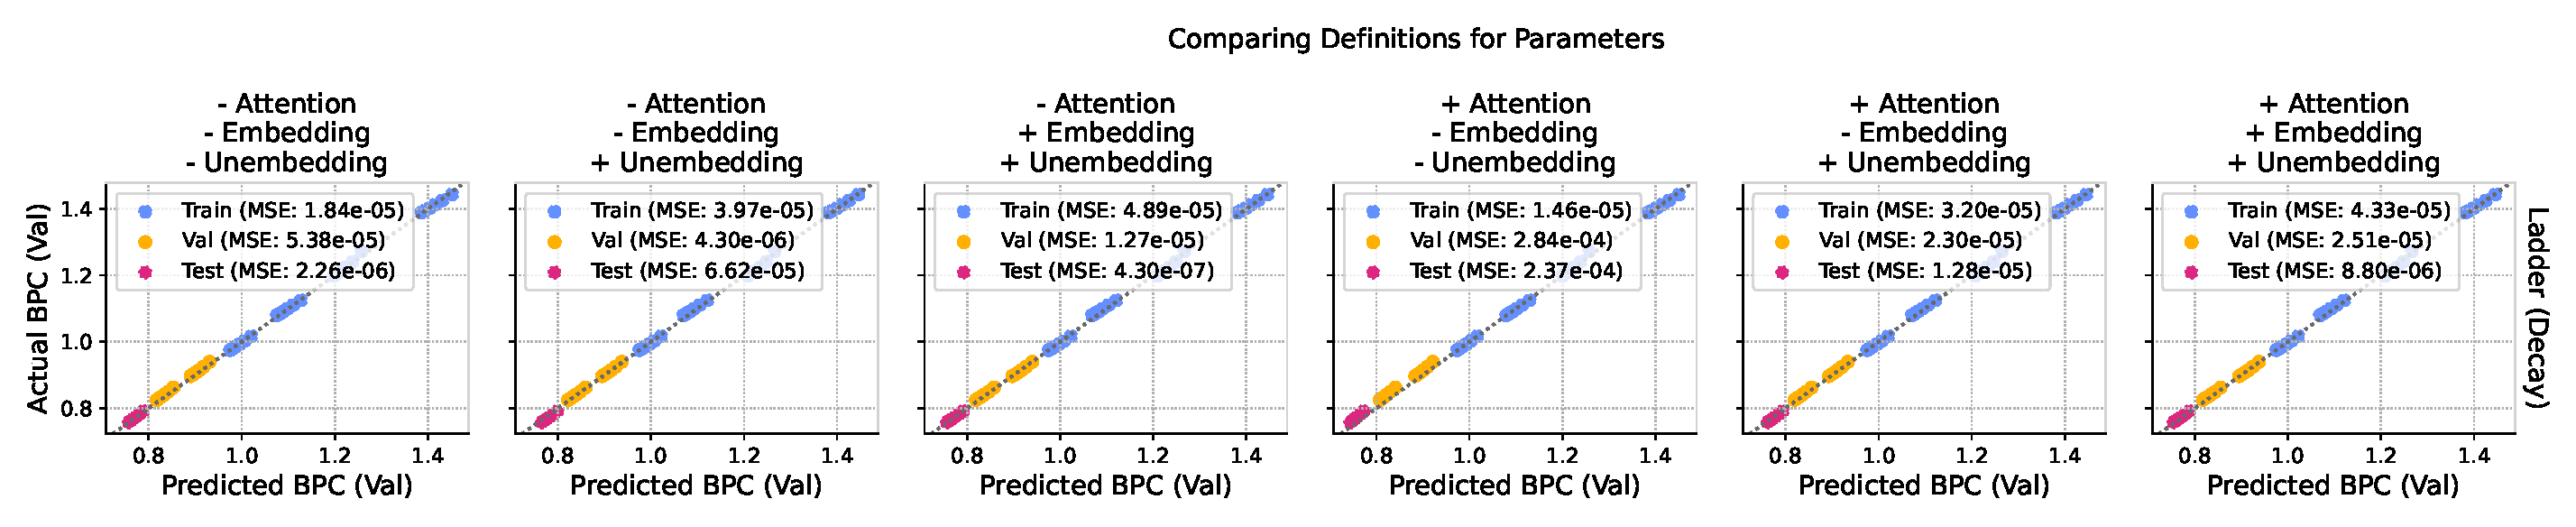
\includegraphics[width=\linewidth]{figures/comparing-definitions-of-parameters.pdf}
    \caption{
        \emph{Even at small scales, how you count parameters has limited impact on the scaling law relative to other factors.} Researchers count parameters in different ways, diverging on whether to (1) account for attention's FLOPs (\texttt{Attention}), (2) include the embedding (\texttt{Embedding}), and (3) include the unembedding (\texttt{Unembedding}). The embedding and unembedding have the same number of parameters, giving six distinct counts. Each one yields a reasonable scaling law.
    }
    \label{fig:comparing-definitions-for-parameters}
\end{figure}

\paragraph{Parameter definitions only make a small difference.} When it comes to scaling laws, researchers define parameters many different ways \citep{Kaplan2020ScalingLaws, Hoffmann2022AnEmpirical, deepseekai2024deepseekllmscalingopensource}. These definitions differ along three axes: whether to account for attention, the embedding, and the unembedding \citep[\S B]{Porian2024Resolving}. The disagreement pivots on the importance of parameters vs. compute: attention uses more FLOPs on longer contexts, while the embedding layer uses no FLOPs at all. \Cref{fig:comparing-definitions-for-parameters} reveals these differences in philosophy lead to little difference in outcome. We use the effective parameters (\texttt{Attention} and \texttt{Unembedding}, no \texttt{Embedding}) as it corresponds most directly to FLOPs per token, keeping $c = 6pd$ exact.

\begin{figure}[b!]
    \centering
    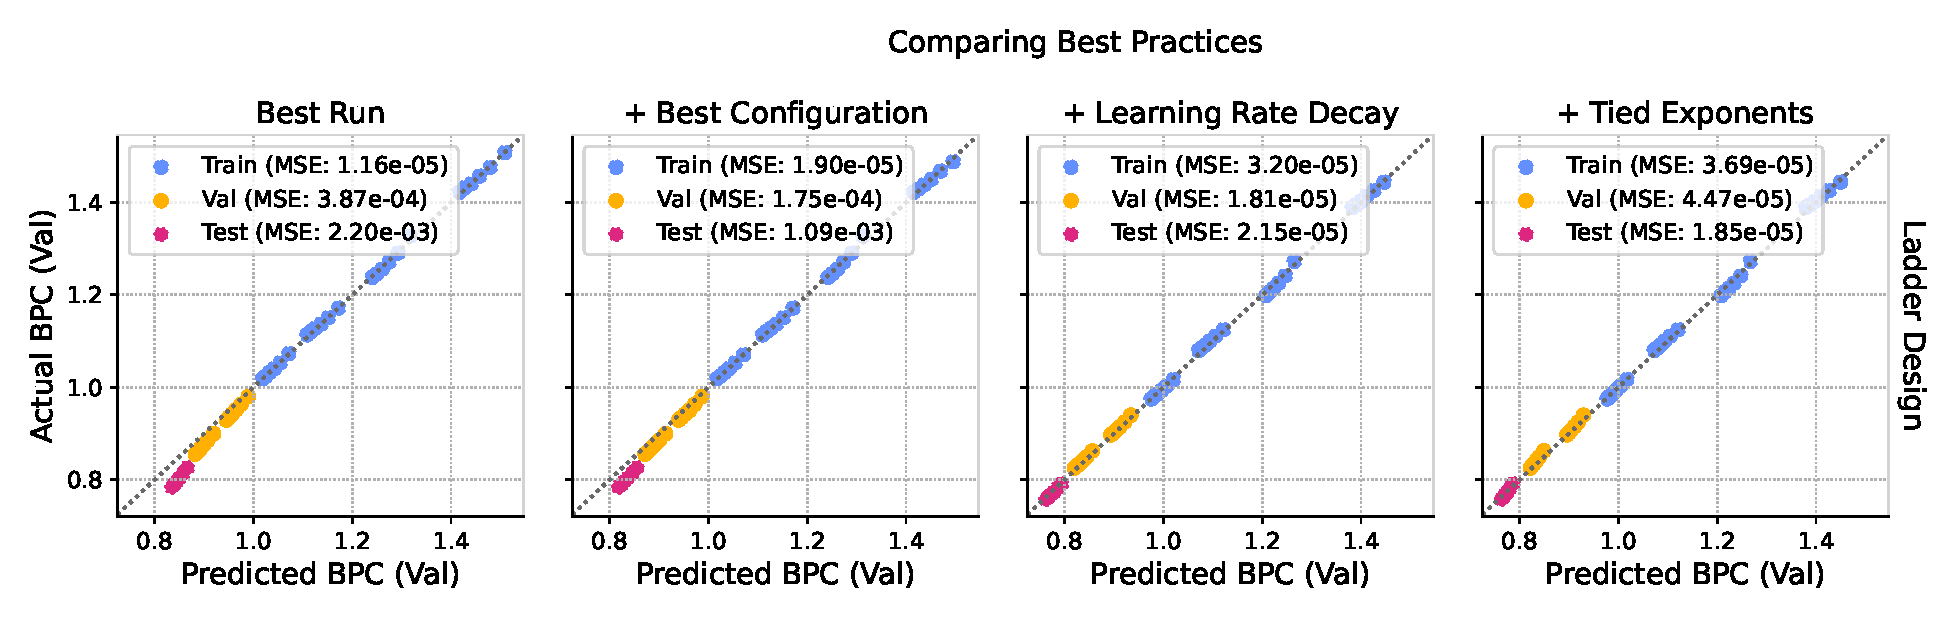
\includegraphics[width=\linewidth]{figures/comparing-best-practices.pdf}
    \caption{
        \emph{Better methodology improves the scaling law, but does not make or break it.} A recognizable law emerges from the outset and extrapolation steadily improves as we move from fitting the best run at each scale (left), to the best configuration for each parameter--data budget (middle left), to decaying the learning rate (middle right). Unlike the other refinements, tying the exponents (right) gives inconsistent results: it slightly improves test but hurts validation.
    }
    \label{fig:comparing-best-practices}
\end{figure}

\paragraph{Other choices refine the estimate, rather than enable it.} \Cref{fig:comparing-best-practices} compares increasing refinements on a basic approach. Fitting the best run at each scale without learning rate decay, the scaling law is immediately recognizable (if imprecise). Improving the methodology refines its precision: tuning hyperparameters for each parameter--data budget reduces test MSE by 50\%, while decaying the learning rate reduces it by a dramatic 98\%. In contrast, tying the exponents ($\iota = \kappa$) makes little difference. The improvements are important for obtaining a good law from small-scale experiments, but even without them the law is present.

\subsection{The Importance of Hyperparameter Tuning}
\label{sec:estimating-small-scale-scaling-laws:the-importance-of-hyperparameter-tuning}

\begin{figure}[t!]
    \centering
    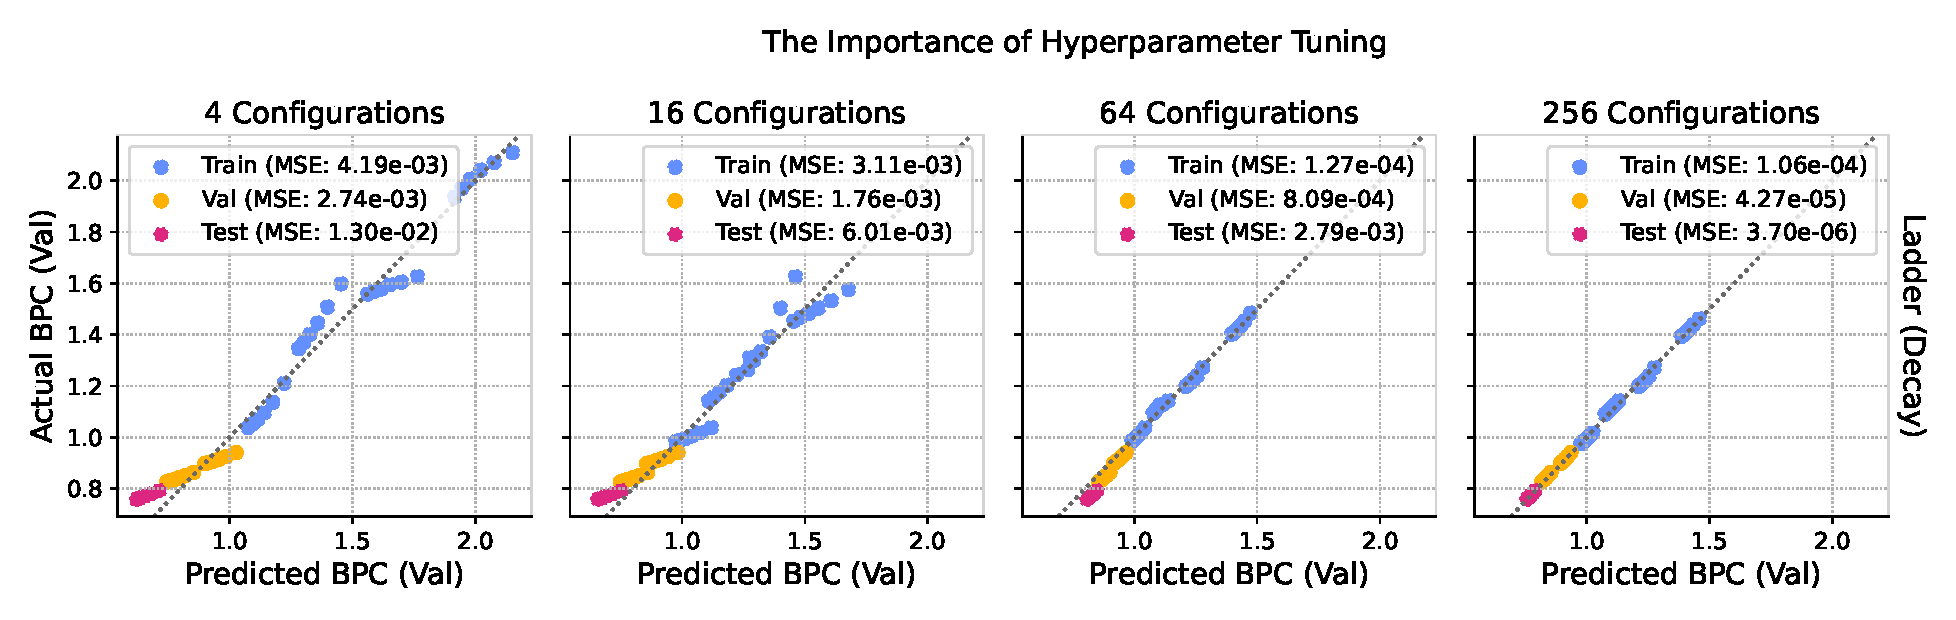
\includegraphics[width=\linewidth]{figures/the-importance-of-hyperparameter-tuning.pdf}
    \caption{
        \emph{Hyperparameter tuning is the single most important step in estimating a scaling law.} Each panel fits a scaling law with a more substantial sweep; all panels evaluate (\texttt{val} and \texttt{test}) on the best configurations from our entire sweep. With 4 (left) or 16 configurations (middle left), the law is not even visible. Increasing to 64 (middle right), it clearly emerges but is imprecise. Only at 256 configurations (right) do we obtain an accurate law.
    }
    \label{fig:the-importance-of-hyperparameter-tuning}
\end{figure}

\Cref{fig:the-importance-of-hyperparameter-tuning} shows what happens with too little tuning effort. With 4 configurations per scale, the scaling law is completely absent. With 16, the scaling law has yet to fully appear; it cannot be estimated reliably as the suboptimal configurations inject too much noise. At 64, the law is clearly visible though extrapolation is weak. Only at 256 configurations do we obtain an accurate scaling law. In our previous study, each refinement improved precision on an already recognizable law; here, with too few configurations there is nothing to fit.

Thus one ingredient above all is required to estimate a scaling law, rigorous hyperparameter tuning. This fact explains why small-scale laws are so easy to miss: uncovering them demands a search far more extensive than most ever run. But why are small models so much more sensitive to their hyperparameters? We will show this change in sensitivity comes from how the hyperparameter loss surface evolves as models scale.

